\documentclass[utf8x, 14pt]{G7-32} %размер бумаги устанавливаем А4, шрифт 14 пунктов

% Остальные стандартные настройки убраны в preamble-std.tex
\sloppy

% 1. Настройки стиля ГОСТ 7-32
% Для начала определяем, хотим мы или нет, чтобы рисунки и таблицы нумеровались в пределах раздела, или нам нужна сквозная нумерация.
% А не забыл ли автор букву 't' ?
\EqInChapter % формулы будут нумероваться в пределах раздела
\TableInChapter % таблицы будут нумероваться в пределах раздела
\PicInChapter % рисунки будут нумероваться в пределах раздела

% 2. Добавляем гипертекстовое оглавление в PDF
\usepackage[
bookmarks=true, colorlinks=true, unicode=true,
urlcolor=black,linkcolor=black, anchorcolor=black,
citecolor=black, menucolor=black, filecolor=black,
]{hyperref}

% 3. Изменение начертания шрифта --- после чего выглядит таймсоподобно.
% apt-get install scalable-cyrfonts-tex

\IfFileExists{cyrtimes.sty}
    {
        \usepackage{cyrtimespatched}
    }
    {
        % А если Times нету, то будет CM...
    }


% 4. Прочие полезные пакеты.
\usepackage{underscore} % Ура! Теперь можно писать подчёркивание.
                        % И нельзя использовать подчёркивание в файлах.
                        % Выбирай, но осторожно.

\usepackage{graphicx}   % Пакет для включения рисунков
\usepackage{pdfpages} % Пакет для включения pdf файлов
\usepackage[utf8x]{inputenc}
\usepackage{lscape} % Меняем ориентацию страницы
\usepackage{rotating}
\usepackage{array}
\usepackage{multicol}
\usepackage{longtable}
\usepackage{multirow}

\newcolumntype{x}[1]
{>{\raggedright}p{#1}}
\newcommand{\tn}{\tabularnewline}

 % 5. Любимые команды
\newcommand{\Code}[1]{\textbf{#1}}

% 6. Поля
% С такими оно полями оно работает по-умолчанию:
% \RequirePackage[left=20mm,right=10mm,top=20mm,bottom=20mm,headsep=0pt]{geometry}
% Если вас тошнит от поля в 10мм --- увеличивайте до 20-ти, ну и про переплёт не забывайте:
\geometry{right=20mm}
\geometry{left=30mm}


% 7. Tikz
\usepackage{tikz}
\usetikzlibrary{arrows,positioning,shadows}

% 8 Листинги

\usepackage{listings}

% Значения по умолчанию
\lstset{
  basicstyle= \footnotesize,
  breakatwhitespace=true,% разрыв строк только на whitespacce
  breaklines=true,       % переносить длинные строки
%   captionpos=b,          % подписи снизу -- вроде не надо
  inputencoding=utf8x,
  keepspaces = true,     % чтобы не удалялись пробелы в русских коментариях
  extendedchars=false,
  numbers=left,          % нумерация слева
  numberstyle=\footnotesize,
  showspaces=false,      % показывать пробелы подчеркиваниями -- идиотизм 70-х годов
  showstringspaces=false,
  showtabs=false,        % и табы тоже
  stepnumber=1,
  tabsize=2,              % кому нужны табы по 8 символов?
  frame=single,
  language=Java
}

% Стиль для псевдокода: строчки обычно короткие, поэтому размер шрифта побольше
\lstdefinestyle{pseudocode}{
  basicstyle=\small,
  keywordstyle=\color{black}\bfseries\underbar,
  language=Pseudocode,
  numberstyle=\footnotesize,
  commentstyle=\footnotesize\it
}

% Стиль для обычного кода: маленький шрифт
\lstdefinestyle{realcode}{
  basicstyle=\scriptsize,
  numberstyle=\footnotesize
}

% Стиль для коротких кусков обычного кода: средний шрифт
\lstdefinestyle{simplecode}{
  basicstyle=\footnotesize,
  numberstyle=\footnotesize
}

% Стиль для BNF
\lstdefinestyle{grammar}{
  basicstyle=\footnotesize,
  numberstyle=\footnotesize,
  stringstyle=\bfseries\ttfamily,
  language=BNF
}

% Определим свой язык для написания псевдокодов на основе Python
\lstdefinelanguage[]{Pseudocode}[]{Python}{
  morekeywords={each,empty,wait,do},% ключевые слова добавлять сюда
  morecomment=[s]{\{}{\}},% комменты {а-ля Pascal} смотрятся нагляднее
  literate=% а сюда добавлять операторы, которые хотите отображать как мат. символы
    {->}{\ensuremath{$\rightarrow$}~}2%
    {<-}{\ensuremath{$\leftarrow$}~}2%
    {:=}{\ensuremath{$\leftarrow$}~}2%
    {<--}{\ensuremath{$\Longleftarrow$}~}2%
}[keywords,comments]

% Свой язык для задания грамматик в BNF
\lstdefinelanguage[]{BNF}[]{}{
  morekeywords={},
  morecomment=[s]{@}{@},
  morestring=[b]",%
  literate=%
    {->}{\ensuremath{$\rightarrow$}~}2%
    {*}{\ensuremath{$^*$}~}2%
    {+}{\ensuremath{$^+$}~}2%
    {|}{\ensuremath{$|$}~}2%
}[keywords,comments,strings]

% Подписи к листингам на русском языке.
\renewcommand*\thelstnumber{\oldstylenums{\the\value{lstnumber}}}
\renewcommand\lstlistingname{\cyr\CYRL\cyri\cyrs\cyrt\cyri\cyrn\cyrg}
\renewcommand\lstlistlistingname{\cyr\CYRL\cyri\cyrs\cyrt\cyri\cyrn\cyrg\cyri}

% Произвольная нумерация списков.
\usepackage{enumerate}


\begin{document}

\includepdf[pagecommand=\thispagestyle{empty}]{import/title} %вставляю pdf титульник, сгенерированный из вордовского файла

\frontmatter % выключает нумерацию ВСЕГО; здесь начинаются ненумерованные главы: реферат, введение, глоссарий, сокращения и прочее

% Команды \breakingbeforechapters и \nonbreakingbeforechapters
% управляют разрывом страницы перед главами.
% По-умолчанию страница разрывается.

% \nobreakingbeforechapters
% \breakingbeforechapters

% Также можно использовать \Referat, как в оригинале
\begin{abstract}
В этой работе ...
\end{abstract}


\tableofcontents

\Defines
\begin{description}
\item[Фреймворк] в информационных системах структура программной системы; программное обеспечение, облегчающее
разработку и объединение разных компонентов большого программного проекта.
\item[Apache JMeter] инструмент для тестирования программного обеспечения, разрабатываемый Apache Jakarta Project.
\item[Java] объектно-ориентированный язык программирования, разработанный компанией Sun Microsystems
(в последующем, приобретённой компанией Oracle).
\item[BlazeDS] серверная Java-технология для передачи данных.
\item[Flex] технология для создания RIA, разработанная компанией Adobe.
\item[Maven] средство для автоматизации сборки проектов.
\item[Прокси-сервер] служба (комплекс программ) в компьютерных сетях, позволяющая клиентам выполнять косвенные
запросы к другим сетевым службам.
\item[Проприетарное программное обеспечение] программное обеспечение, являющееся частной собственностью авторов или
правообладателей и не удовлетворяющее критериям свободного ПО.
\end{description}

\Abbreviations %% Список обозначений и сокращений в тексте
\begin{description}
\item[RIA] Rich Internet application, приложения, доступные через сеть Интернет, обладающие особенностями и
функциональностью традиционных настольных приложений.
\item[Flex] технология для создания RIA, разработанная компанией Adobe.
\item[AMF] Action Message Format, бинарный формат обмена данными.
\item[Фреймворк] в информационных системах структура программной системы; программное обеспечение, облегчающее
разработку и объединение разных компонентов большого программного проекта.
\item[Apache JMeter] инструмент для тестирования программного обеспечения, разрабатываемый Apache Jakarta Project.
\item[Java] объектно-ориентированный язык программирования, разработанный компанией Sun Microsystems
(в последующем, приобретённой компанией Oracle).
\item[BlazeDS] серверная Java-технология для передачи данных.
\item[Maven] средство для автоматизации сборки проектов.
\end{description}


\Introduction % * - чтобы не нумеровалось

Данный дипломный проект ориентирован на практическое применение навыков автоматизации тестирования:
обзор и анализ существующих методов и средств нагрузочного тестирования, разработку программного обеспечения,
в значительной степени снижающего сложность осуществления функционального и нагрузочного тестирования
взаимодействия клиента и сервера по AMF-протоколу.

В настоящее время активно развивается рынок Web-приложений. Все больше различных услуг 
предоставляется через Интернет, классические информационные системы в различных компаниях
также становятся Web-приложениями, предоставляя для своих сотрудников и партнеров
доступ к ресурсам компании не только из локальной, но и из глобальной сети. Концепции
и технологии, используемые при разработке web-приложений, постоянно развиваются и
совершенствуются. Оптимизируется использование ресурсов и времени, улучшаются
возможности по отображению предоставляемой информации, динамичность и интерактивность
web-приложений\cite{overview}.

На сегодняшний день одним из наиболее перспективных подходов к обеспечению всего 
вышеперечисленного является концепция Rich Internet Application (в дальнейшем RIA) - 
это приложения, доступные через сеть Интернет, обладающие особенностями и
функциональностью традиционных настольных приложений.
 
Приложения RIA, как правило:

\begin{enumerate}
\item передают веб-клиенту необходимую часть пользовательского  интерфейса,
оставляя большую часть данных (ресурсы программы, данные и пр.) на сервере;
\item запускаются в браузере и не требуют дополнительной установки программного
обеспечения;
\item запускаются локально в среде безопасности, называемой <<песочница>> (sandbox).
\end{enumerate}

На рис.~\ref{ris:RIAinWorld.png} демонстрируется место Rich Internet Applications
среди других технологий программных систем
\begin{figure}[ht]
\center{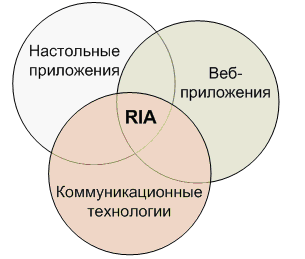
\includegraphics[height=60mm, width=80mm]{fig/intro/RIAinWorld.png}}
\caption{RIA среди других технологий}
\label{ris:RIAinWorld.png}
\end{figure}

Термин «RIA» впервые был упомянут компанией Macromedia в официальном сообщении в
марте 2002 года\cite{modeling3}. Подобные концепции существовали и несколькими годами ранее, например:

\begin{enumerate}
\item DHTML --- HTML страницы с динамическим содержимым;
\item Java-applet --- это программы написанные на языке Java, как правило, предназначенные для загрузки посредством
браузера;
\end{enumerate}

Для начала рассмотрим архитектурные особенности построения web-приложений базирующихся 
на RIA концепции. Для этого сравним принцип работы традиционного web-приложения и
RIA-приложения (Рис.~\ref{ris:principlesRIA.png}).
\begin{figure}[ht]
\center{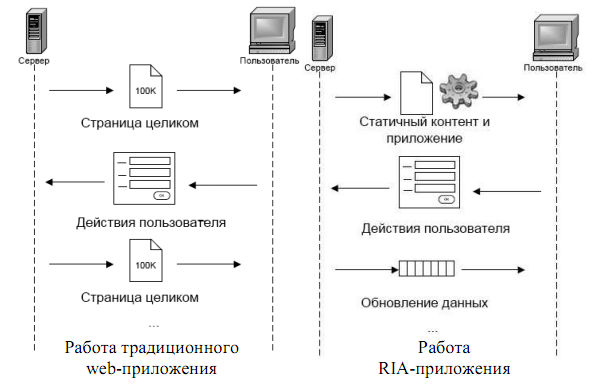
\includegraphics[height=80mm, width=100mm]{fig/intro/principlesRIA.png}}
\caption{Принципы работы традиционного web-приложения и RIA приложения}
\label{ris:principlesRIA.png}
\end{figure}

Работа традиционных web-приложений сконцентрирована вокруг клиент серверной архитектуры 
с тонким клиентом. Такой клиент переносит все задачи по обработке информации на сервер,
а сам используется в основном для отображения статического контента. Основной
недостаток этого подхода в том, что все взаимодействие с приложением должно
обрабатываться сервером, что требует постоянной отправки данных на сервер,
ожидания ответа сервера, и загрузки страницы обратно в браузер. В отличие от 
традиционного web-приложения в RIA значительная часть функциональности исполняется на
стороне клиента, поэтому появляется возможность отправлять и получать данные с сервера
только по мере необходимости\cite{modeling1}. Если подключение нестабильно, клиентская часть RIA-
приложения обладает возможностями кэширования данных и работы без подключения к сети в 
режиме offline.

На основе вышесказанного, можно выделить ряд преимуществ RIA как перед настольными приложения,
так и перед стандартными веб-приложениями:

\begin{enumerate}
\item для работы с RIA не требуется установка приложения, как правило, все что необходимо, это установка плагина
для браузера;
\item пользователи могут использовать приложение на любом компьютере, имеющем соединение с Интернет,
причем обычно не важно, какая операционная система на нем установлена;
\item интерфейс RIA обладает большей интерактивностью, он не ограничен лишь использованием языка
HTML, применяемого в стандартных веб-приложениях. Наиболее сложные приложения RIA предлагают 
внешний вид и функциональность, близкие к настольным приложениям;
\item при работе веб-приложения компьютер пользователя гораздо меньше подвержен риску
вирусному заражению, чем при запуске исполняемых бинарных файлов;
\item использование вычислительных ресурсов клиента и сервера лучше сбалансировано;
\item взаимодействие клиента с сервером осуществляется без ожидания каких-либо действий
пользователя.
\end{enumerate}

Для реализации RIA многими IT-компаниями предлагаются различные технологии. Наиболее известными из 
них являются AJAX, Flash, Flex (в дальнейшем Flex) и AIR фирмы Adobe; ActiveX, WPF и Silverlight
корпорации Microsoft; Java FX и Java Applets компании Sun Microsystems.

В настоящее время одной из наиболее распространенных технологий разработки RIA является Adobe Flex,
которая представляет собой среду с открытым кодом для создания и обслуживания web-приложений,
совместимую со всеми распространенными браузерами, платформами персональных компьютеров и версиями
операционных систем и имеющую максимальную поддержку со стороны разработчиков\cite{modeling2}.

Flex представляет собой набор классов, расширяющих возможности Flash. Flex позволяет описывать
интерфейс web-приложения на MXML – декларативном языке описания и настройки свойств визуальных 
элементов интерфейса, основанном на XML. Логика web-приложения пишется на ActionScript – полноценном
объектно-ориентированном языке программирования, который является одним из диалектов ECMAScript.
Результатом компиляции является файл SWF, предназначенный для выполнения в браузере (на платформе
Flash Player, которая существует в виде плагина к браузеру) или как самостоятельное приложение (на
платформе AIR).

Flex-framework включает возможности локализации, стилизации приложения, разработки модульного приложения, 
встроенные валидаторы и форматоры текстовых полей --- все те инструменты, которые нужны разработчикам
приложений, работающих online. Также Flex предоставляет полные мультимедийные возможности Flash 
Platform, такие как потоковое мультимедиа, возможность получить доступ к веб-камере и микрофону
пользователя, бинарные сокеты, обширные возможности сетевых коммуникаций (HTTP-запросы, веб-сервисы, 
встроенный формат сериализации AMF), оперирование координатами трехмерного пространства).

Вся разработка во Flex ориентирована на применение готового набора расширяемых компонентов,
внешний вид которых позволяет гибко настраивать CSS, что облегчает задачу разработчика.

Flex SDK является бесплатным инструментарием с июня 2007 года с открытым исходным кодом,
распространяемым на условиях Mozilla Public License. Для работы с процедурами и классами этого фреймворка
можно использовать как бесплатные (Eclipse WTP IDE, FlashDevelop IDE) так и платные
(Flex Builder IDE, IntelliJ IDEA IDE, Aptana Studio IDE, PowerFlasher FDT IDE) среды разработки.

Flex приложения предоставляют возможность реализации клиент-серверного взаимодействия 
на основе бинарного формата обмена данными --- AMF (Action Message Format). AMF
используется для сериализации структурированных данных, таких как объекты Action Script 
или XML, и обмена сообщениями между Adobe Flash клиентом и удалённым сервисом. AMF более
экономичен по трафику по сравнению с XML и позволяет передавать типизированные объекты.

Как известно огромную роль в жизненном цикле программного обеспечения играет фаза тестирования.
Тестирование программного обеспечения — проверка соответствия между реальным и ожидаемым поведением программы,
осуществляемая на конечном наборе тестов, выбранном определенным образом. Существует множество подходов
к решению задачи тестирования и видов их классификации. По объекту тестирования чаще всего
используется следующее разделение:

\begin{enumerate}
\item Функциональное тестирование;
\item Тестирование производительности;
\begin{enumerate}
\item Нагрузочное тестирование;
\item Стресс-тестирование;
\item Тестирование стабильности;
\end{enumerate}
\item Юзабилити-тестирование;
\item Тестирование интерфейса пользователя;
\item Тестирование безопасности;
\item Тестирование локализации;
\item Тестирование совместимости;
\end{enumerate}

На практике для тестирования клиент-серверных приложений чаще всего применяются функциональное и нагрузочное
тестирование.

Функциональное тестирование рассматривает заранее указанное поведение и основывается на анализе спецификаций
функциональности компонента или системы в целом. Функциональные тесты основываются на функциях, выполняемых системой,
и могут проводиться на всех уровнях тестирования (компонентном, интеграционном, системном, приемочном). Как правило,
эти функции описываются в требованиях, функциональных спецификациях или в виде случаев использования системы (use cases).

Нагрузочное тестирование — определение или сбор показателей производительности и времени отклика
программно-технической системы или устройства в ответ на внешний запрос с целью установления соответствия требованиям,
предъявляемым к данной системе (устройству). Основная цель нагрузочного тестирования заключается в том, чтобы, создав
определённую ожидаемую в системе нагрузку (например, посредством виртуальных пользователей) и, обычно, использовав
идентичное программное и аппаратное обеспечение, наблюдать за показателями производительности системы.

Важным этапом фазы тестирования является автоматизация тестов. Автоматизированное тестирование использует программные средства для
выполнения тестов и проверки их результатов, что помогает сократить
время тестирования и упростить его процесс, а также может 
дать возможность выполнять определенные тестовые задачи намного быстрее и 
эффективнее чем это может быть сделано вручную. Автоматизация тестирования 
даёт следующие преимущества\cite{dot-com}:

\begin{enumerate}
\item Выполнение сложно воспроизводимых вручную тестов, таких как нагрузочное
и стресс-тестирование;
\item Меньшие затраты на поддержку --- когда автоматические скрипты уже написаны, на их поддержку
и анализ результатов требуется, как правило, меньшее время чем на проведение того же объема тестирования вручную;
\item Повторяемость --- все написанные тесты всегда будут выполняться однообразно, то есть
исключен «человеческий фактор». Тестировщик не пропустит тест по неосторожности и ничего не
напутает в результатах;
\item Быстрое выполнение --- автоматизированному скрипту не нужно сверяться с инструкциями и
документациями, это сильно экономит время выполнения;
\item Отчеты --- автоматически рассылаемые и сохраняемые отчеты о результатах тестирования.
\end{enumerate}

Если сложить все вышесказанное, то больший объем тестирования, может быть
достигнут с меньшими усилиями, давая при этом возможность улучшать как качество, 
так и продуктивность\cite{testing}.

Однако использование AMF вызывает ряд трудностей для реализации автоматизации функционального 
и нагрузочного тестирования взаимодействия сервера и Flex клиента, связанных с бинарной 
природой протокола. Так как amf является бинарным,
разработчикам и тестировщикам трудно считывать и изменять содержащуюся в нём информацию.

Отдельной проблемой является нагрузочное тестирование таких приложений, а именно имитация работы с
приложением большого количества пользователей за счёт запуска набора тестов в несколько потоков. 
Сложность состоит в поддержке уникальности идентификатора сессии каждого клиента. Идентификатор 
клиента выделяется строго одному подключенному SWF-файлу и прошит в передаваемых данных.
Стандартный порядок тестирования --- запись запросов пользователя с использованием прокси-сервера
и запуск сохранённого сценария в несколько потоков --- в данном случае будет неэффективным, так
как все перехваченные запросы будут иметь одинаковый идентификатор клиента и тесты пройдут
только в 1 потоке, а остальные будут возвращены с ошибкой о неправильной сессии.
 
Таким образом, можно сформулировать наличие противоречия между необходимостью проведения функционального
и нагрузочного тестирования и сложностью его реализации на технологии Flex и поставить следующие задачи на
дипломную работу:

\begin{enumerate}
\item разработка программного обеспечения, в значительной степени снижающего сложность осуществления функционального
и нагрузочного тестирования взаимодействия клиента и сервера по AMF-протоколу;
\item разработка методики функционального и нагрузочного тестирования с использованием предложенного ПО.
\end{enumerate}% это введение

\mainmatter % это включает нумерацию глав и секций в документе ниже

\chapter{Анализ существующих решений}
 
На сегодняшний день существует ряд различных программных комплексов, предоставляющих
возможность для проведения функционального, нагрузочного, регрессионного 
тестирования различного рода приложений. Проведём обзор наиболее распространённых и доступных утилит и
укажем их функционал по обеспечению тестирования в области Flex технологий.

\section{Обзор утилит для тестирования Flex приложений}

\subsection{HP QuickTest Professional}

HP QuickTest Professional (QTP) — один из инструментов автоматизации 
функционального тестирования, является флагманским продуктом компании 
HP в своей линейке. Для разработки автоматизированных тестов QTP 
использует язык VBScript(Visual Basic Scripting Edition ) — скриптовый 
язык программирования, интерпретируемый компонентом Windows Script Host.
Он широко используется при создании скриптов в операционных системах
семейства Microsoft Windows. QTP поддерживает ряд технологий, среди
которых есть и Macromedia Flex. Поддержка Flex осуществляется засчёт
установки плагина, предоставляемого компанией Adobe (Flex QTP add-in).

Чтобы приступить к тестированию приложение необходимо скомпилировать, 
создав для него HTML-оболочку, и развернуть его либо локально, либо на 
web-сервере. Создание тестов в QTP осуществляется следующим образом:
приложение открывается в браузере и все действия, совершаемые пользователем с 
пользовательским интерфейсом приложения записываются в виде строчек Visual Basic скрипта. 
QTP поддерживает запись большинства наиболее часто используемых во Flex 
приложениях событий (операций), связанных с пользовательским интерфейсом. 
Однако часть из них, например некоторые атомарные операции, игнорируются 
во время записи тестов. Пользователь имеет возможность добавить их в 
текст скрипта вручную. Для проверки правильности выполнения теста 
пользователь задаёт ожидаемые значения для выполняемых операций ---
checkpoints. Во время автоматического прогона тестов запускать браузер 
уже не нужно, достаточно лишь указать HTML страницу, используемую для 
тестов. Для выявления причины возникновения ошибок в тестах или каких-либо 
других неполадок можно обратиться к логам Flash Player или настроить и 
включить логирование в QTP. Возможность прогона тестов в несколько потоков
в QTP отсутствует

Для проведения тестов с HP QuickTest Professional необходимо использовать
 браузер Internet Explorer версии 6 или выше. HP QuickTest Professional 
работает с операционными системами семейства Windows и является платным 
программным обеспечением.

\subsection{IBM Rational Functional Tester}

IBM Rational Functional Tester является средством автоматизированного 
регрессивного тестирования, предназначенным для тестирования Java, .NET, 
Web-приложений, включая Flex-приложения, и терминальных приложений на 
платформах Windows и Linux\cite{ibmfuctional}. Functional Tester поддерживает два языка
сценариев: Java и Visual Basic.NET. Для тестирования Java-приложений в 
программу Functional Tester включена открытая среда разработки Eclipse. 
Установка дополнительных компонентов не требуется. Если требуется 
использовать язык сценариев Visual Basic.NET, перед установкой IBM 
Rational Functional Tester необходимо установить Visual Studio.NET.

Перед началом тестирования приложение загружается в браузере, затем все 
действия,совершаемые пользователем записываются в виде Java или Visual 
Basic.NET скрипта (в зависимости от настроек). Пользователь может 
редактировать скрипты, а также задавать ожидаемые результаты выполнения 
той или иной операции для проверки работы приложения. Как и QTP, IBM 
Rational Functional Tester во время записи тестов добавляет компоненты 
приложения в свой набор объектов. Далее тесты можно запускать в 
автоматическом режиме. Также в IBM Rational Functional Tester имеется 
возможность многократного запуска тестов с различным набором данных. 
Если стандартного набора объектов(таких как кнопки, текстовые поля и т.д.) 
недостаточно, существует возможность самостоятельно добавить во фреймворк 
необходимые объекты. Это возможно благодаря Rational Functional Tester 
proxy software development kit (SDK), который имеет удобное API и 
довольно подробную сопроводительную документацию.
Также IBM Rational Functional Tester упрощает механизм регрессионного 
тестирования. Functional Tester использует усовершенствованную технологию 
ScriptAssure для того, чтобы «изучить» контрольные характеристики 
пользовательского интерфейса, что позволяет идентифицировать те же самые 
средства управления в новой версии, несмотря на внесенные изменения. 
Эти характеристики сохраняются в объектной карте, совместный доступ к 
которой могут получить различные скрипты и участники проекта. 
Благодаря этой карте изменения, внесенные в характеристики распознавания 
объекта, будут отражены во всех скриптах тестирования, что существенно 
упрощает обслуживание. 

Rational Functional Tester поддерживает операционные системы Windows 
2000, XP, Vista, 7, Linux. Является платным программным обеспечением.

\subsection{NeoLoad}

NeoLoad --- профессиональный инструмент нагрузочного тестирования веб-приложений,
в том числе и Flex, работающий на многих платформах, в том числе Windows, Solaris, Linux.
Осуществляя моделирование большого числа пользователей, которые обращаются 
к приложению, NeoLoad делает проверку надежности и производительности 
приложения при разных нагрузках.

Тестирование Flex приложений осуществляется засчёт записи AMF трафика во 
время взаимодействия пользователя с приложением. Все перехваченные запросы 
отображаются в xml формате, что позволяет редактировать содержащиеся в них 
данные. Далее записанные тесты могут быть запущены в несколько потоков.

NeoLoad является платным программным обеспечением с закрытым исходным кодом. 
 
\subsection{Apache JMeter}

JMeter --- инструмент для проведения нагрузочного тестирования, изначально
разрабатывался как средство тестирования web-приложений, в настоящее время 
он способен проводить нагрузочные тесты для JDBC-соединений, FTP, LDAP, SOAP, 
JMS, POP3, IMAP, HTTP и TCP. 
В JMeter реализованы возможность создания большого количества запросов с 
помощью нескольких компьютеров при управлении этим процессом с одного из них,
логирование результатов тестов и разнообразная визуализация результатов в
виде диаграмм, таблиц и т. п.

Ключевое понятие в JMeter –-- план тестирования. План тестирования приложения
представляет собой описание последовательности шагов, которые
будет исполнять JMeter. План тестирования может содержать:

\begin{enumerate}
\item Группы потоков (Thread Groups) --- элемент, позволяющий конфигурировать
многопоточный запуск тестов
\item Контроллеры --- позволяют создаватьтесты со сложной логической структурой.
\item Слушатели --- отображают результаты выполнения тестов
\item Соответствия --- позволяют сравнивать полученные результаты с
ожиданиями пользователя
\item Сэмплеры --- основные элемнты тест-плана, в которых формируется тело
запроса, тестовый шаг.
\end{enumerate}

На данный момент в JMeter нет отдельных средств для тестирования Flex приложений, 
однако есть возможность записи http запросов, содержащих в себе тело AMF 
сообщения, с помощью прокси-сервера. Далее перехваченные запросы могут быть 
перенесены в план тестирования и запущены в режиме нагрузочного тестирования. 
Созданные в JMeter тесты могут быть запущены с помощью систем сборок проектов Maven и 
Ant. Также JMeter свободно интегрируется со многими серверами сборок, такими как Jenkins 
и Hudson.

JMeter является бесплатным кросс-платформенным Java-приложением с открытым
исходным кодом и удобным API. Существует большое количество плагинов к JMeter, 
значительно расщиряющих его базовую функциональность.

\chapter{Программная реализация модуля}

\section{Выбор технического средства решения задачи}

\section{Руководство пользователя}

\subsection{Установка JMeter}

Для начала необходимо скачать с сайта производителя zip архив, содержащий все необходимы для установки файлы,
а затем распаковать его на диске. Место установки JMeter далее будем называть JMETER\_HOME.

\subsection{Установка модуля amf-translator}

Чтобы подключить к JMeter модуль amf-translator, достаточно добавить jar-файл приложения в каталог JMETER\_HOME/lib/ext.

\subsection{Запуск приложения}

Приложение запускается с помощью файла jmeter.bat или ApacheJMeter.jar, находящихся в каталоге JMETER\_HOME/bin.

\subsection{Настройка прокси-сервера}

После запуска в окне приложения с левой стороны нам доступно дерево элементов. Чтобы создать прокси сервер
с поддержкой протокола AMF, необходимо правой кнопкой мыши кликнуть по элементу WorkBench,
а затем добавить элемент AMF Proxy Server (WorkBench > Add > Non-Test Elements > AMF Proxy Server).

\begin{figure}[ht]
\center{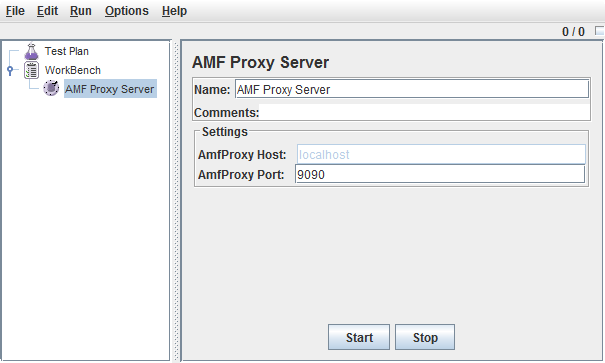
\includegraphics[height=120mm, width=160mm]{fig/development/proxySettings.png}}
\caption{Настройка прокси-сервера}
\label{ris:proxySettings.png}
\end{figure}

В поле AmfProxy Port необходимо указать номер порта, который будет слушать наш прокси сервер.
Если указать, например, 9090, то прокси-сервер будет запущен на localhost:9090.
Затем точно такие же настройки прокси-сервера устанавливаются в браузере, с помощью которого будет
производиться тестирование. Также стоит убедиться, что указанный Вами порт уже не занят другим приложением.

\subsection{Запись тестового сценария}

После того, как в AMF Proxy Server установлены все необходимые параметры, нажимается кнопка Start,
запускающая прокси-сервер.

\begin{figure}[h]
\center{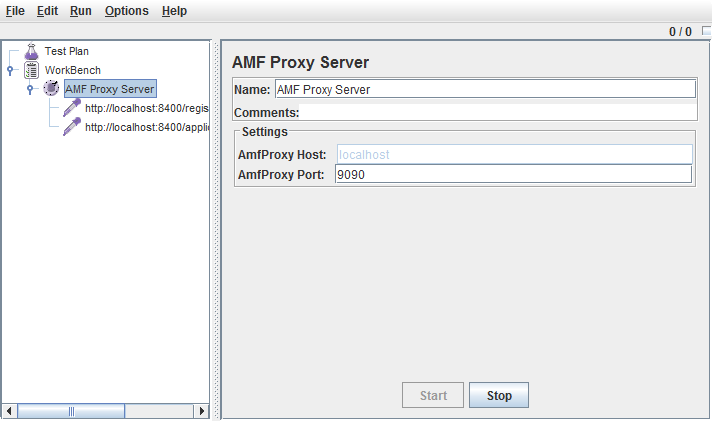
\includegraphics[height=120mm, width=160mm]{fig/development/proxyStart.png}}
\caption{Запуск прокси-сервера}
\label{ris:proxyStart.png}
\end{figure}

Затем тестируемое приложение открывается в браузере, для которого также
применены соответсвующие настройки прокси-сервера, и пользователь может выполнять с Flex приложением
необходимые операции, которые будут записываться AMF Proxy Server в виде элементов AMF RPC Sampler и в
дальнейшем могут быть перенесены в тест-план. Чтобы завершить запись тестовых запросов, необходимо
нажать кнопку Stop. После завершения записи тестов, все перехваченные запросы отображаются в дереве
элементов JMeter в качестве дочерних элементов AMF Proxy Server.

\subsection{Создание тест-плана}

Создание тест-плана в JMeter осуществляется следующим образом.
В первую очередь добавляется группа потоков - Thread Group (Test Plan > Threads (Users) > Thread Group).

\begin{figure}[ht]
\center{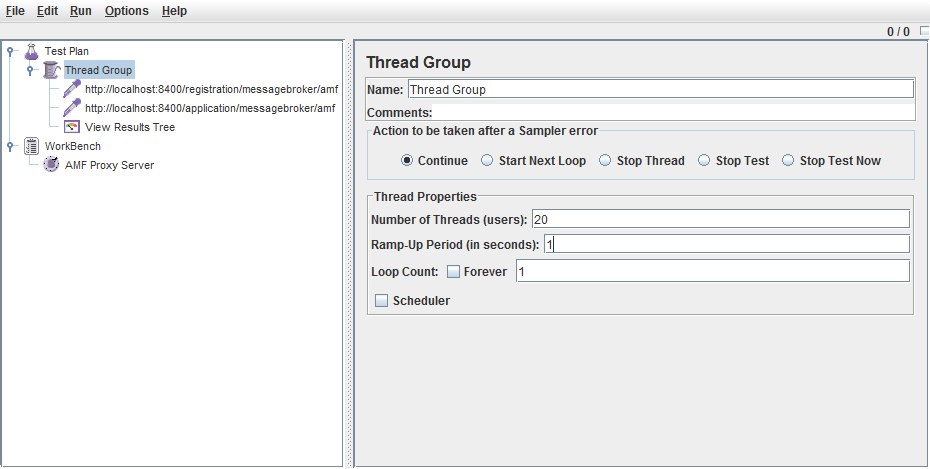
\includegraphics[height=120mm, width=160mm]{fig/development/testplan.png}}
\caption{Создание тест-плана}
\label{ris:testplan.png}
\end{figure}

Этот элемент является ключевым в тест-плане JMeter, именно его функционал отвечает за реализацию
нагрузочного тестирования --- многопоточного запуска последовательности тестовых шагов.
В данном элементе задается следующее:

\begin{enumerate}
\item Действия, которые будут производиться в случае, если в тест выполняется с ошибкой
(Action to be taken after a Sampler error);
\item Число потоков, в которое будут запускаться шаги тест-плана (Number of Threads);
\item Интервал, в течение которого будет запущено указанное в предыдущем параметре
число потоков (Ramp-Up Period);
\item Число повторений набора тестов (Loop Count);
\item Расписание запуска тестов (Scheduler).
\end{enumerate}

Затем в Thread Group в качестве дочерних элементов добавляются шаги тестов, которые
будут запускаться с указанными характеристиками. В нашем случае мы переносим элементы
AMF RPC Sampler, записанные с помощью прокси.

AMF RPC Sampler представляет собой форму для вызова процедур java-объектов на стороне
сервера. Чтобы вызвать метод удалённого объекта, необходимо заполнить следующие
поля: 

\begin{enumerate}
\item Endpoint Url - URL, по которому отправляется запрос
\item AMF Call - имя удалённого объекта и процедуы, которая должна быть вызвана; 
Например, если мы хоти вызвать у объекта registrationDestionation метод registerUser, 
в этом поле следует написать registrationDestination.registerUser;
\item Request Parameters - параметры метода, вызываемого у объекта (если они 
существуют).
\end{enumerate}

На Рис.~\ref{ris:amfSampler.png} представлен интерфейс AMF RPC Sampler.
\begin{figure}[ht]
\center{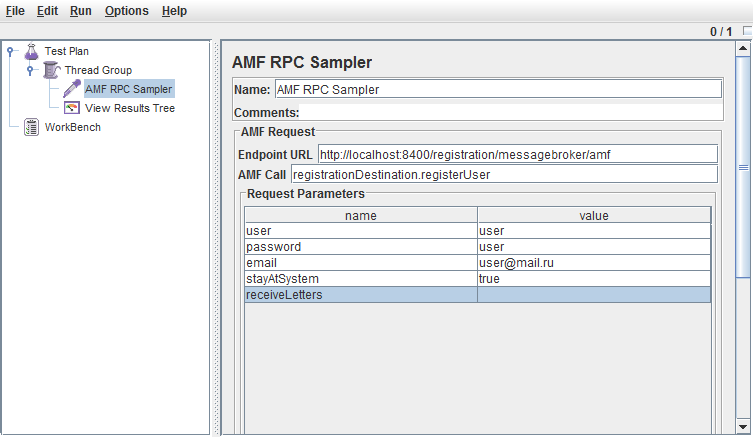
\includegraphics[height=120mm, width=160mm]{fig/development/amfSampler.png}}
\caption{Интерфейс элемента AMF RPC Sampler}
\label{ris:amfSampler.png}
\end{figure}
 
Помимо сэмплера в тест-план также следует добавить визуалайзер результатов, чтобы иметь возможность
отслеживать ход тестового сценария (Thread Group > Add > Listener ).
JMeter предлагает большой выбор таких элементов, для примера будем использовать View Results Tree.
После того как план сформирован, он может быть сохранён. (File > Save Test Plan As...)

\subsection{Запуск тестов}

Чтобы запустить содержимое элемента Test Plan, необходимо выбрать в основном меню Run > Start.
После заврешения прогона тестов результаты их выполнения можно наблюдать в View Results Tree.

\begin{figure}[ht]
\center{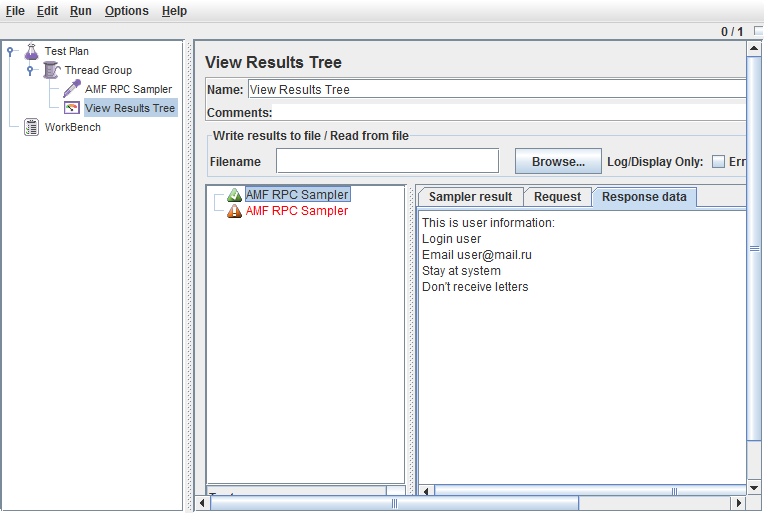
\includegraphics[height=110mm, width=160mm]{fig/development/testResults.png}}
\caption{Отображение результатов тестов в визуалайзере View Results Tree}
\label{ris:testResults.png}
\end{figure}

В правой части визуалайзера отображается дерево элементов тест плана и статус 
их выполнения - если элемент подсвечен зелёным цветом, то шаг выполнен 
успешно, если красным - то нет. Также на вкладках слева предоставляется 
возможность просмотра отправленного запроса и полученного от сервера ответа.  

\section{Методика тестирования}
\chapter{Технико-экономическое обоснование}

\section{Концепция экономического обоснования}

На сегодняшний день одним из наиболее перспективных направлений в разработке
web-приложений является концепция Rich Internet Application (в дальнейшем RIA) --- это приложения,
доступные через сеть Интернет, обладающие особенностями и функциональностью традиционных настольных приложений.
Одной из наиболее распространенных технологий разработки RIA является Adobe Flex.
Flex приложения предоставляют возможность реализации клиент-серверного взаимодействия на основе бинарного формата
обмена данными --- AMF(Action Message Format). AMF более экономичен по трафику по сравнению с XML и позволяет
передавать типизированные объекты.
Как известно огромную роль в жизненном цикле программного обеспечения играет фаза тестирования.
Автоматизированное тестирование является его составной частью. Оно использует программные средства для
выполнения тестов и проверки их результатов, что помогает сократить время тестирования и упростить его процесс,
а также может дать возможность выполнять определенные тестовые задачи намного быстрее и эффективнее чем это может
быть сделано вручную. Однако использование AMF вызывает ряд трудностей для реализации автоматизации
функционального и нагрузочного тестирования взаимодействия сервера и Flex клиента, связанных с
бинарной природой протокола. Так как amf сообщение представляет собой совокупность байтов, разработчикам
и тестировщикам трудно считывать и изменять содержащуюся в нём информацию. Отдельной проблемой является
нагрузочное тестирование таких приложений --- имитация работы с приложением большого количества пользователей
за счёт запуска набора тестов в несколько потоков. Выходом из сложившейся ситуации является разработка
программного обеспечения, в значительной степени снижающего сложность осуществления функционального и
нагрузочного тестирования взаимодействия клиента и сервера по AMF-протоколу, а также разработка
методики функционального и нагрузочного тестирования использованием предложенного ПО.

Целью технико-экономического обоснования является определение экономической целесообразности реализации проекта.
Этапами ТЭО являются:

\begin{enumerate}
\item трудоемкость и календарный план выполнения НИР;
\item смета затрат на проведение НИР;
\item комплексная оценка эффективности НИР.
\end{enumerate}

\section{Рынок и план маркетинга}

\subsection{Сегментирование рынка}

Сегментирование рынка состоит в выделении сегментов анализируемого рынка и оценки спроса
на продукцию в каждом сегменте рынка.

Итак, выделим основные сегменты:
\begin{enumerate}
\item Компании, осуществляющие разработку программного обеспечения.
\item Компании, специализирующиеся на внешнем тестировании программного обеспечения.
\item Программисты, осуществляющие разработку ПО в частном порядке (для личных или коммерческих целей).
\end{enumerate}

Проведем анализ требований различных групп потенциальных покупателей к продукции:
\begin{enumerate}
\item технический уровень, качество и надежность в эксплуатации, уровень послепродажного обслуживания;
\item технический уровень, качество и надежность в эксплуатации, уровень послепродажного обслуживания;
\item цена продукции, качество и надежность в эксплуатации.
\end{enumerate}

\subsection{Продвижение товара}
Для эффективного продвижения товара, а так же для поддержания спроса необходима реклама, предоставление скидок,
 демо-версии для привлечения новых клиентов. Поскольку продукт является специализированным, следует давать 
 рекламу в журналы, газеты, размещать на сайтах и форумах той же тематики. Скидки, как правило, стимулируют 
 уже существующих клиентов, поскольку важно, привлекая новых, не потерять уже существующих пользователей.

\subsection{Производство продукта}

Проводится расчет затрат, связанных с проведением НИР. Основные статьи калькуляции приведены ниже:
\begin{enumerate}
\item Материалы
\item Спецоборудование
\item Расходы на оплату труда
\item Отчисления на социальные нужды
\item Затраты по работам, выполняемым сторонними организациями
\item Командировочные расходы
\item Прочие прямые расходы
\item Накладные расходы
\end{enumerate}

\subsection{Статья <<Материалы>>}

На статью относятся затраты на сырье, основные и вспомогательные материалы, покупные  полуфабрикаты
и комплектующие изделия, необходимые для выполнения конкретной НИР c учетом транспортно-заготовительных
расходов. Калькуляция расходов по статье «Материалы» приведена в табл.~\ref{tab:material}.

\begin{table}[ht]
\caption{Материалы}
\begin{tabular}{|c|c|c|c|}
\hline
Наименование материалов&Коли-чество, шт&Цена, р.&Сумма, р.\\
\hline
Бумага формата А4&1&120&120\\
\hline
Заправка картриджа для принтера&1&300&300\\
\hline
Записываемый диск CD-RW&1&50&50\\
\hline
\multicolumn{3}{|r|}{Итого:}&470\\
\hline
\multicolumn{3}{|r|}{Транспортные расходы, 15\%:}&70\\
\hline
\multicolumn{3}{|r|}{Всего:}&540\\
\hline
\end{tabular}
\label{tab:material}
\end{table}

\subsection{Статья <<Спецоборудование>>}

На статью <<Спецоборудование>> относятся затраты на приобретение (или изготовление) специальных приборов,
стендов, другого специального оборудования, необходимого для выполнения конкретной НИР.
Для данной НИР дополнительного спецоборудования не требуется.

\subsection{Статья <<Расходы на оплату труда>>}

На статью относится заработная плата научных сотрудников, инженеров и прочего инженерно-технического персонала,
непосредственно занятых выполнением конкретной НИР. Эти расходы складываются из основной и дополнительной
заработной платы. Средняя зарплата за один рабочий день определяется, исходя из месячного оклада и среднего
количества рабочих дней за месяц, принимаемого за 22 дня.\\
Основная зарплата рассчитывается по формуле:

\begin{equation}
C_{зо} = \frac{T \cdot C_{зо.мес}}{22}\mbox{,}
\label{F:F1}
\end{equation}

где Т – трудоемкость выполнения работ по НИР, $С_{зо.мес}$ – месячный оклад.\\
Дополнительная зарплата рассчитывается по формуле:

\begin{equation}
C_{зд} = \frac{C_{зо} \cdot Н_{д}}{100}\mbox{,}
\label{F:F2}
\end{equation}

где $C_{зо}$ – основная зарплата, $Н_{д}$ – норматив дополнительной зарплаты.\\
Производим расчет основной и дополнительной зарплат на основании следующих данных:

\begin{enumerate}
\item трудоемкость выполнения работ исполнителем $Т_{исп}$ = 106~чел.-дн.;
\item трудоемкость выполнения работ СНС $Т_{рук}$= 7~чел.-дн.;
\item месячный оклад инженера $С_{зо.мес.исп}$ = 15~000~р.;
\item месячный оклад руководителя $С_{зо.мес.рук}$ = 20~000~р.;
\item норматив дополнительной зарплаты $Н_{д}$ = 12\%.
\end{enumerate}

%\begin{equation}
\begin{align}
&С_{зо.исп} = \frac{106 \cdot 15 000}{22} = 72 272 р.\mbox{,}\\
&С_{зо.рук} = \frac{7 \cdot 20 000}{22} = 6 363 р.\mbox{,}\\
&С_{зо} = 72 272 + 6 363 = 78 635 р.\mbox{,}\\
&С_{зд.исп} = \frac{72 272 \cdot 12}{100} = 8 672 р.\mbox{,}\\
&С_{зд.рук} = \frac{6 363 \cdot 12}{100} = 763 р.\mbox{,}\\
&С_{зд} = 8 672 + 763 = 9 435 р.
\end{align}
%\end{equation}

Общие расходы на оплату труда составляют 88 070 р.

\subsection{Статья <<Отчисления на социальные нужды>>}

На статью относят затраты, связанные с выплатой единого социального налога.
Данная статья рассчитывается пропорционально зарплате в размере 26,2\%:
\begin{enumerate}
\item федеральный бюджет – 20\%;
\item фонд социального страхования – 3.2\%;
\item фонд обязательного медицинского страхования – 2,8\%;
\item страхование от несчастных случаев – 0,2\%.
\end{enumerate}

\begin{equation}
C_{зд} = \frac{P_{от} \cdot Н_{сн}}{100}\mbox{,}
\label{F:F3}
\end{equation}

где $Н_{сн}$ – суммарный норматив отчислений на социальные нужды – 26,2%.

\begin{equation}
С_{сн} = \frac{88070 \cdot 26,2}{100} = 23 074 р.\mbox{,}
\label{F:F4}
\end{equation}

\subsection{Статья <<Затраты  по работам, выполняемым сторонними организациями>>}

Расходов на работы, выполняемые сторонними организациями, не существует.

\subsection{Статья <<Командировочные расходы>>}

На статью относятся расходы на все виды служебных командировок работников, выполняющих
задания по конкретной НИР. В данной НИР расходов, связанных со служебными командировками, нет.

\subsection{Статья <<Прочие прямые расходы>>}

На статью относятся расходы на получение специальной научно-технической информации, платежи
за использование средств связи и коммуникации, а также другие расходы, необходимые для проведения НИР.
На всех этапах работы требуется выход в Интернет. Стоимость работы в Интернете составляет 350~р. в месяц.
Затраты на Интернет на весь период составляют:

\begin{equation}
С_{и} = \frac{350}{22} \cdot 106 = 1 686 р.\mbox{,}
\label{F:F5}
\end{equation}

Также требуется использование телефона. Примем эти расходы ориентировочно равными $С_{т}$ = 300 р.
Следовательно, суммарно прочие прямые затраты составляют:

\begin{equation}
С_{ппз} = С_{и} + С_{т} = 1 686 + 300 = 1 986 р.\mbox{,}
\label{F:F6}
\end{equation}

\subsection{Статья <<Накладные расходы>>}

В статью включаются расходы на управление и хозяйственное обслуживание НИР.

\begin{equation}
С_{нр} = \frac{P_{от} \cdot H_{нр}}{100}\mbox{,}
\label{F:F5}
\end{equation}

где $Н_{нр}$ – норма накладных расходов, равная 20\%.

\begin{equation}
С_{нр} = 88 070 \cdot \frac{20}{100} = 17 614 р.
\label{F:F5}
\end{equation}

На основании полученных данных в табл.~\ref{tab:calc} приведена калькуляция себестоимости разработки.

\begin{table}[ht]
\caption{Смета затрат на проведение НИР}
\begin{tabular}{|c|p{10cm}|c|}
\hline
№ п/п&Наименование статьи&Сумма, р.\\
\hline
1&Материалы&540\\
\hline
2&Спецоборудование&---\\
\hline
3&Расходы на оплату труда&88070\\
\hline
4&Отчисления на социальные нужды&23074\\
\hline
5&Затраты по работам, выполняемым сторонними организациями&---\\
\hline
6&Командировочные расходы&---\\
\hline
7&Прочие прямые расходы&1986\\
\hline
8&Накладные расходы&17614\\
\hline
\multicolumn{2}{|r|}{Себестоимость НИР:}&131 284\\
\hline
\end{tabular}
\label{tab:calc}
\end{table}

\section{Организационный план проекта}

\begin{landscape}
\begin{longtable}{|c|c|c|c|c|c|c|c|c|c|c|c|c|c|c|c|c|c|c|c|c|c|c|c|c|c|c|c|c|c|}
\caption{Трудоемкость и календарный план выполнения НИР}
\label{tab:longtable}
\\ \hline
\multirow{2}{*}{№}&\multirow{2}{*}{Этапы и работы}&\multicolumn{2}{|c|}{Трудоемкость, чел.-дн.}&\multirow{2}{*}{Численность, чел.}&\multirow{2}{*}{Длительность, дн.}&\multicolumn{24}{|c|}{Продолжительность работы (пятидневка)}\\\cline{3-4}\cline{7-30}
&&Исполнитель&Руководитель НИР&&&4&9&14&19&24&29&33&36&41&46&47&52&53&58&59&64&69&74&78&83&86&91&111&113\\\cline{3-4}\cline{7-30}
\hline \endfirsthead
\subcaption{Продолжение таблицы~\ref{tab:longtable}}
\\ \hline \endhead
\hline \subcaption{Продолжение на след. стр.}
\endfoot
\hline \endlastfoot
1& • & • & • & • & • & • & • & • & • & • & • & • & • & • & • & • & • & • & • & • & • & • & • & • & • & • & • & • & • \\
\hline 
2& • & • & • & • & • & • & • & • & • & • & • & • & • & • & • & • & • & • & • & • & • & • & • & • & • & • & • & • & • \\
\hline 
3 & • & • & • & • & • & • & • & • & • & • & • & • & • & • & • & • & • & • & • & • & • & • & • & • & • & • & • & • & • \\
\hline 
4 & • & • & • & • & • & • & • & • & • & • & • & • & • & • & • & • & • & • & • & • & • & • & • & • & • & • & • & • & • \\
\hline 
5 & • & • & • & • & • & • & • & • & • & • & • & • & • & • & • & • & • & • & • & • & • & • & • & • & • & • & • & • & • \\
\hline 
6 & • & • & • & • & • & • & • & • & • & • & • & • & • & • & • & • & • & • & • & • & • & • & • & • & • & • & • & • & • \\
\hline 
7 & • & • & • & • & • & • & • & • & • & • & • & • & • & • & • & • & • & • & • & • & • & • & • & • & • & • & • & • & • \\
\hline 
8 & • & • & • & • & • & • & • & • & • & • & • & • & • & • & • & • & • & • & • & • & • & • & • & • & • & • & • & • & • \\
\hline 
9 & • & • & • & • & • & • & • & • & • & • & • & • & • & • & • & • & • & • & • & • & • & • & • & • & • & • & • & • & • \\
\hline 
10 & • & • & • & • & • & • & • & • & • & • & • & • & • & • & • & • & • & • & • & • & • & • & • & • & • & • & • & • & • \\
\hline 
11 & • & • & • & • & • & • & • & • & • & • & • & • & • & • & • & • & • & • & • & • & • & • & • & • & • & • & • & • & • \\
\hline 
12 & • & • & • & • & • & • & • & • & • & • & • & • & • & • & • & • & • & • & • & • & • & • & • & • & • & • & • & • & • \\
\hline 
13 & • & • & • & • & • & • & • & • & • & • & • & • & • & • & • & • & • & • & • & • & • & • & • & • & • & • & • & • & • \\
\hline 
14 & • & • & • & • & • & • & • & • & • & • & • & • & • & • & • & • & • & • & • & • & • & • & • & • & • & • & • & • & • \\
\hline 
15 & • & • & • & • & • & • & • & • & • & • & • & • & • & • & • & • & • & • & • & • & • & • & • & • & • & • & • & • & • \\
\hline 
16 & • & • & • & • & • & • & • & • & • & • & • & • & • & • & • & • & • & • & • & • & • & • & • & • & • & • & • & • & • \\
\hline 
16 & • & • & • & • & • & • & • & • & • & • & • & • & • & • & • & • & • & • & • & • & • & • & • & • & • & • & • & • & • \\
\hline
16 & • & • & • & • & • & • & • & • & • & • & • & • & • & • & • & • & • & • & • & • & • & • & • & • & • & • & • & • & • \\
\hline
16 & • & • & • & • & • & • & • & • & • & • & • & • & • & • & • & • & • & • & • & • & • & • & • & • & • & • & • & • & • \\
\hline
16 & • & • & • & • & • & • & • & • & • & • & • & • & • & • & • & • & • & • & • & • & • & • & • & • & • & • & • & • & • \\
\hline
16 & • & • & • & • & • & • & • & • & • & • & • & • & • & • & • & • & • & • & • & • & • & • & • & • & • & • & • & • & • \\
\hline
16 & • & • & • & • & • & • & • & • & • & • & • & • & • & • & • & • & • & • & • & • & • & • & • & • & • & • & • & • & • \\
\hline
\end{longtable}
\end{landscape}

Трудоемкость выполнения работы исполнителем  составляет 106 чел.-дней, а руковолителем 7 чел.-дней.
Общая продолжительность выполнения данной НИР 113 дней (чуть больше 15 недель).

\section{Комплексная оценка эффективности НИР}

\subsection{Научно-технический эффект разработки}

Концепции и технологии, используемые при разработке web-приложений,
постоянно развиваются и совершенствуются - оптимизируется использование ресурсов и времени,
улучшаются возможности по отображению предоставляемой информации, динамичность и их интерактивность.

Flex является одним из самых распространённых и перспективных инструментов разработки web-приложений.
Разрабатываемый в дипломном проекте программный модуль поможет обеспечить контроль качества Flex
приложений, а также повысит эффективность тестирования за счёт автоматизации тестовых сценариев.

\subsection{Экономический эффект}

Выгоды, которые может получить потребитель от использования разрабатываемой продукции:

\begin{enumerate}
\item Повышение стабильности разрабатываемого приложения за счёт обеспечения качественного тестирования.
\item Повышение скорости тестирования за счёт автоматизации труда инженеров по качеству.
\item Понижение затрат на тестирование, т.к. внедрение разрабатываемого модуля позволяет отказаться от
использования платных средств автоматизированного тестирования.
\end{enumerate}

\subsection{Расчет потребности в начальных инвестициях}

Потребность в начальном капитале определяется средствами, израсходованных на НИР – 131 284 р.,
a также дополнительными средствами, необходимых для приобретения ПЭВМ и принтера. При стоимости ПЭВМ 20 000 р.,
сроке ее службы – 5 лет, времени копирования программного обеспечения 0,5 ч. потребность в ПЭВМ составит:
\chapter{Охрана интеллектуальной собственности}

\section{Интеллектуальная собственность}

Согласно определению интеллектуальной собственности, принятому в российском законодательстве,
а также на основании определения Стокгольмской конференции от 14 июля 1967 г., компьютерные программы
относятся к объектам интеллектуальной собственности. Компьютерным программам предоставляется охрана
нормами авторского права как литературным произведениям в соответствии с Бернской конвенцией.
В Российской Федерации вопросы предоставления правовой охраны программам регулируются Гражданским
кодексом РФ, Часть~4~(ГК~РФ~Ч.4).

\section{Программа для ЭВМ}

Под программой для ЭВМ понимается <<... представленная в объективной форме совокупность данных и команд,
предназначенных для функционирования ЭВМ и других компьютерных устройств в целях получения определенного
результата>>. Кроме того, в понятие программы для ЭВМ входят <<...подготовительные материалы, полученные
в ходе разработки программы для ЭВМ, и порождаемые ею аудиовизуальные отображения>>~[2,~ст.~1261].
С точки зрения программистов и пользователей программа для ЭВМ представляет собой детализацию алгоритма
решения какой-либо задачи и выражена в форме определенной последовательности предписаний, обеспечивающих
выполнение компьютером преобразования исходных данных в искомый результат.

Можно выделить следующие объективные формы представления программы для ЭВМ:
\begin{enumerate}
\item исходная программа (или исходный текст) --- последовательность предписаний на алгоритмическом языке
высокого уровня, предназначенных для автоматизированного перевода этих предписаний в последовательность команд
в объектном коде;
\item рабочая программа (или объектный код) --- последовательность машинных команд, т. е. команд, представленных
на языке, понятном ЭВМ;
\item программа, временно введенная в память ЭВМ, --- совокупность физических состояний элементов памяти
запоминающего устройства ЭВМ (ОЗУ), сохраняющихся до прекращения подачи электропитания к ЭВМ;
\item программа, постоянно хранимая в памяти ЭВМ, --- представленная на языке машины команда (или серия команд),
выполненная в виде физических особенностей участка интегральной схемы, сохраняющихся независимо от подачи
электропитания.
\end{enumerate}

Исходная и рабочая программы представляются в электронном виде.
Правовая охрана программ для ЭВМ распространяется только в отношении формы их выражения и <<… не распространяется
на идеи, концепции, принципы, методы, процессы, системы, способы, решения технических, организационных или иных
задач, открытия, факты, языки программирования>>~[2,~ст.1259,~п.~5].

\section{Авторское право на программу для ЭВМ}

Предпосылкой охраноспособности программы для ЭВМ и базы данных является их творческий характер, т. е. они
должны быть продуктом личного творчества автора. Творческий характер деятельности автора предполагается до
тех пор, пока не доказано обратное~[2,~ст.~1257].

Момент возникновения авторского права является важнейшим юридическим фактом, который устанавливается в силу
создания программы для ЭВМ. <<Для возникновения, осуществления и защиты авторских прав не требуется регистрация
произведения или соблюдение каких-либо иных формальностей>>~[2,~ст.1259,~п.4].

Закон устанавливает, что обнародование программы не является обязательным условием для возникновения прав на нее:
<<Авторские права распространяется как на обнародованные, так и на необнародованные произведения, выраженные в
какой-либо объективной форме ...>>~[2,~ст.~1259,~п.~3].

Таким образом, только сам факт создания программы, зафиксированной в объективной форме, является основанием
возникновения авторского права на нее.

Каждая составляющая понятия использования программы для ЭВМ имеет конкретное содержание, которое также
определено законом:
\begin{enumerate}
\item воспроизведение --- <<... изготовление одного или более экземпляров произведения или его части
в любой материальной форме, … в том числе запись в память ЭВМ>>~[2,~ст.~1270,~п.~2,~п.п.1];
\item распространение –-- предоставление доступа к произведению <<... путем продажи или иного отчуждения его
оригинала или экземпляров>>~[2,~ст.~1270,~п.~2,~п.п.2];
\item публичный показ --- <<... любая демонстрация оригинала или экземпляров произведения непосредственно ...
либо с помощью технических средств в месте, открытом для свободного посещения, или в месте, где присутствует
значительное число лиц ...>>~[2,~ст.~1270,~п.~2,~п.п.3].
\end{enumerate}

В целях оповещения о своих правах правообладатель <<... вправе использовать знак охраны авторского права,
который помещается на каждом экземпляре произведения и состоит из следующих элементов:
латинской буквы С в окружности; имени или наименования правообладателя; года первого опубликования
произведения>>~[2,~ст.~1271].

Исключительные права на программу переходят по наследству в установленном законом порядке, и их можно
реализовать в течение срока действия авторского права.

Передача прав на материальный носитель не влечет за собой передачи каких-либо прав на программу для
ЭВМ~[2,~ст.1227]. Иными словами, передача носителя информации (например, диска) с зафиксированной на
нем программой третьему лицу не означает передачи каких-либо прав на эту программу.

\section{Правообладание}

Если человек (или группа людей) самостоятельно, по личной инициативе создал программу для ЭВМ,
то он является одновременно и автором, и правообладателем созданного произведения, что позволяет ему по
собственному усмотрению использовать эту программу (или базу данных) в личных целях, продавать, раздавать
бесплатно, разрешать тиражировать и распространять или иным образом распоряжаться своими исключительными правами.

Кроме личных (неимущественных) прав автору “служебной” программы для ЭВМ (базы данных) принадлежит
право на вознаграждение при условии использования работодателем созданных произведений или передачи
исключительного права другому лицу. Размер и порядок выплаты этого определяется договором~[2,~ст.~1295,~п.~2].

\section{Нарушение прав на программу для ЭВМ и базу данных}

Специфика программ для ЭВМ такова, что они очень уязвимы в смысле их незаконного использования
(прежде всего, путем копирования и распространения копий). Незаконно изготовленные (скопированные)
или используемые экземпляры программы для ЭВМ или базы данных называются контрафактными, а
несанкционированное использование чужих программ или баз данных путем опубликования (выпуска в свет),
воспроизведения (полного или частичного), распространения, иного использования считается нарушением
исключительных прав на программы для ЭВМ или базы данных, т. е. нарушением авторского права.

\section{Право на официальную регистрацию}

В ст.~1262~ГК~РФ~Ч.4 закреплено право автора или иного правообладателя на государственную регистрацию
программы для ЭВМ или базы данных: <<Правообладатель в течение срока действия исключительного права
на программу для ЭВМ может по своему желанию зарегистрировать такую программу для ЭВМ или такую базу данных
в федеральном органе исполнительной власти по интеллектуальной собственности>>.
Исключение составляют программы для ЭВМ и базы данных, в которых содержатся сведения, составляющие
государственную тайну.

Предусмотренная регистрация не является правообразующей и носит факультативный характер,
т. е. с ней не связано возникновение прав на программу для ЭВМ, однако такая процедура представляется
полезной по следующим соображениям.

\begin{enumerate}
\item Она является официальным уведомлением общественности о наличии у правообладателей прав в
отношении рассматриваемых объектов.
\item Государственная регистрация содействует защите прав в случае возникновения конфликтных ситуаций
при нарушении прав или установлении приоритета.
\end{enumerate}

\section{Процедура официальной регистрации}

Процедура официальной регистрации программ для ЭВМ и баз данных в целом определена ст.~1262~ГК~РФ~Ч.4 и
включает подачу заявки в федеральный орган исполнительной власти по интеллектуальной собственности (Роспатент),
проверку поданных документов и собственно регистрацию. После поступления заявки на регистрацию в Роспатент
проверяется наличие необходимых документов и их соответствие установленным требованиям. При положительном
результате проверки сведения о программе для ЭВМ или базе данных вносятся, соответственно, в Реестр программ
для ЭВМ или Реестр баз данных под уникальным регистрационным номером и выдается заявителю (здесь заявителем
называют правообладателя, подавшего заявку на регистрацию программы или базы данных в Роспатент) свидетельство
о государственной регистрации установленной формы, в котором указаны регистрационный номер объекта по Реестру,
название программы или базы данных, имя или наименование правообладателя, фамилии авторов и дата регистрации.
Сведения о зарегистрированных программах для ЭВМ и базах данных публикуются в официальном бюллетене Роспатента.

\section{Заявка на официальную регистрацию}

Состав заявки на официальную регистрацию программы для ЭВМ или базы данных (далее - Заявка) определен
п.~2~ст.~1262~ГК~РФ~Ч.1, а также в Правилах составления, подачи и рассмотрения заявок на официальную
регистрацию программ для электронных вычислительных машин и баз данных (далее - Правила).

Заявка должна относиться к одной программе или одной базе данных.
При этом <<Программа для ЭВМ, состоящая из нескольких программ для ЭВМ (программный комплекс),
которые не могут быть использованы самостоятельно, регистрируется в целом (без регистрации каждой
входящей в нее (него) программы для ЭВМ)>>~[3,~п.~5]. Заявка должна содержать следующие документы:
\begin{enumerate}
\item заявление о государственной регистрации;
\item депонируемые материалы, идентифицирующие программу для ЭВМ, включая реферат;
\item документ, подтверждающий уплату государственной пошлины в установленном размере или
основание для освобождения от уплаты государственной пошлины или уменьшения его размера.
\end{enumerate}

В Правилах подробно описаны требования, предъявляемые к документам заявки.

Заявление на официальную регистрацию представляется отпечатанным на типографском бланке или в виде
компьютерной распечатки согласно образцам, приведенным в приложениях к Правилам (формы РП и РП/ДОП).

В состав депонируемых материалов входит также реферат, который представляется в двух экземплярах отдельно
от листинга программы для ЭВМ или описания структуры базы данных и не входит в их объем.
Реферат должен содержать информацию, определенную в п.п.~18а)~---~18и),~п.21~и~п.23~Правил,
в полном объеме. При этом:
\begin{enumerate}
\item аннотация реферата должна содержать сведения, определенные п.~18г)~Правил;
\item объем памяти указывается в Кбайтах или Мбайтах и определяется для программ как объем памяти,
занимаемый исходным текстом программы (листингом).
\end{enumerate}

\section{Программный продукт и формы его продажи}

Программный продукт --- персонифицированная программа для ЭВМ или база данных, которая предназначена
для самостоятельного использования конкретным пользователем в личных целях.

Коммерческая реализация (продажа) программного продукта связана с понятием использования программы для
ЭВМ третьими лицами (пользователями) и осуществляется на основании лицензионного договора с правообладателем.
Договор заключается в письменном виде и может определять следующие условия: способы использования, порядок
выплаты вознаграждения и срок действия договора, а также территорию, на которой используется данный
продукт~[2,~ст.~1235,~1236].

Одним из типов лицензионного договора на программу для ЭВМ является традиционный двухсторонний договор
правообладателя –-- лицензиара, с покупателем (пользователем) --- лицензиатом, в котором определяется
способы, сроки, территория использования программы или базы данных. Такие договоры составляются, как
правило, при единичных продажах программного продукта, предназначенного для решения достаточно узких
прикладных задач (научных, отраслевых и т. п.), при продажах программного продукта, требующего регулярного
обновления и дополнения (некоторые базы данных), а также при передаче прав на тиражирование и
распространение программ для ЭВМ или баз данных.

\section{Договор на использование программы для ЭВМ}

Текст договора должен содержать определенную исчерпывающую формулировку лицензионного соглашения между
владельцем прав на программу для ЭВМ (далее --- объект договора) и покупателем (приобретателем прав
на использование объекта договора).

\backmatter %% Здесь заканчивается нумерованная часть документа и начинаются ссылки и
            %% заключение

\Conclusion

В рамках дипломного проекта был проведён обзор последних тенденций на рынке Web приложений, который
показал востребованность технологии RIA, в частности Flex приложений. Были сформулирваны основные проблемы,
возникающие при тестировании взаимодействия Flex приложений с сервером, на основании которых
поставлено техническое задание. Распространённость технологии
Flex и неотъемлимость фазы тестирования в жизненном цикле программного обеспечения подтверждают
актуальность темы дипломного проекта.

Анализ уже существующих решений по тестированию Flex приложений показал,что ни одно из них в полной мере не
удовлетворяет свормулированным техническим требованиям, в результате чего было принято решение о разработке
собственного программного обеспечения, способного решить поставленную задачу.

Результатом реализации задачи дипломного проекта является программный модуль для тестового фреймворка
Apache JMeter, предоставляющий возможность функционального и нагрузочного тестирования взаимодействия Flex
приложения с сервером через AMF. В качестве серверной технологии используется BlazeDS.

Были проведены работы по модульному и функциональному тестированию разработанного ПО, показавшие его соответствие
заявленным требованиям.

В завершении дипломного проекта было составлено экономическое обоснование и приведен раздел,
посвященный защите интеллектуальной собственности.

Планируется дальнейшее развитие программного модуля с целью улучшения визуализации результатов тестов,
доработки пользовательского интерфейса и поддержки других функций BlazeDS.



% % Список литературы при помощи BibTeX
% Юзать так:
%
% pdflatex diplom
% bibtex diplom
% pdflatex diplom

\bibliographystyle{gost780u}
\bibliography{diplom}


\appendix   % Тут идут приложения

\chapter{Программный код модуля}
\label{cha:appendix1}

\lstinputlisting[caption=Код реализация декодера сообщений]{../../src/main/java/edu/leti/amf/MessageDecoder.java}

\lstinputlisting[caption=Интерфейс обработки http-запросов]{../../src/main/java/edu/leti/jmeter/proxy/SamplerDeliverer.java}

\lstinputlisting[caption=Интерфейс прокси сервера]{../../src/main/java/edu/leti/jmeter/proxy/ProxyInterface.java}

\chapter{План приёмочных испытаний приложения <<Модуль для тестирования взаимодействия Flex приложений с сервером через AMF>>}
\label{cha:appendix2}

\section{Объект тестирования}

Объектом тестирования является программный модуль для тестирования взаимодействия Flex приложений с сервером через
протокол AMF. Модуль является дополнением к тестовому фреймворку Apache JMeter.

\section{Цели и приоритеты тестирования}

Целью тестирования является проверка соответсвия разработанного программного обеспечения требованиям, установленным
в техническом задании.

\section{Стратегии тестирования}

Функциональное тестирование --- проверка соответствия требованиям, указанным в техническом задании,
применяется к функционалу, за который отвечает разрабатываемый модуль.

\section{Последовательность работ}

\begin{enumerate}
\item Проектирование набора тестовых случаев;
\item Подготовка тестового окружения;
\item Проведение тестирования;
\item Анализ результатов;
\end{enumerate}

\section{Критерии начала тестирования}

\begin{enumerate}
\item законченность разработки требуемого функционала;
\item наличие задокументированных требований к программному обеспечению;
\item наличие набора тестовых случаев;
\item готовность тестового окружения;
\end{enumerate}

\section{Критерии окончания тестирования}

\begin{enumerate}
\item соответствие продукта функциональным требованиям;
\item стабильность работы продукта на протяжении обозначенного периода;
\end{enumerate}

\section{Тестовое окружение}

Для проведения тестирования необходимо следующее программное обеспечение:

\begin{enumerate}
\item сервер BlazeDS;
\item скомпилированное Flex приложение, использующее AMF канал для передачи сообщений;
\item web-браузер c установленным Flash Player;
\item Apache JMeter;
\item Apach Maven;
\end{enumerate}

\chapter{Сценарии тестирования приложения}
\label{cha:appendix3}

\section{Настройка тестового окружения}

Перед проведением тестов необходимо настроить тестовую среду следующим образом:

\begin{enumerate}
\item установить программное обеспечение, указанное в разделе "Тестовое окружение" плана приёмочных испытаний.
Место установки JMeter далее будем называть JMETER\_HOME;
\item подключить к JMeter тестируемый модуль amf-translator --- добавить jar-файл приложения в каталог
JMETER\_HOME/lib/ext;
\item развернуть Flex приложение на сервере BlazeDS, запустить его и убедиться, что оно функционирует;
\item запустить JMeter --- приложение запускается с помощью файла jmeter.bat или ApacheJMeter.jar, находящихся в
каталоге JMETER\_HOME/bin.
\end{enumerate}

\section{Функциональные тесты}

\subsection{Проверка записи тестовых запросов}

Предусловия:

\begin{enumerate}
\item Добавить элемент AMF Proxy Server (WorkBench > Add > Non-Test Elements > AMF Proxy Server);

\begin{figure}[ht]
\center{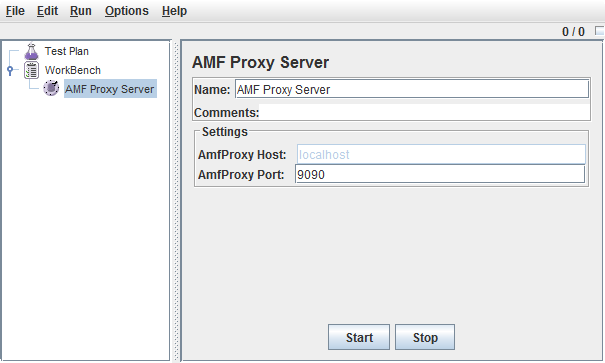
\includegraphics[height=120mm, width=160mm]{fig/development/proxySettings.png}}
\caption{Настройка прокси-сервера}
\label{ris:proxySettings.png}
\end{figure}

\item В поле AmfProxy Port необходимо указать номер порта, который будет слушать наш прокси сервер.
Если указать, например, 9090, то прокси-сервер будет запущен на localhost:9090;
\item Запустить браузер и указать там точно такие же настройки прокси-сервера.
Также стоит убедиться, что указанный Вами порт уже не занят другим приложением;
\item Далее открыть в браузере Flex приложение;
\end{enumerate}

Шаги теста:

\begin{enumerate}
\item Запустить прокси-сервер, нажав кнопку "Start"
\item С помощью браузера ввести данные во Flex приложение и вызвать метод удалённого объект.
\item Завершить запись тестовых запросов, нажав кнопку "Stop"
\end{enumerate}

Ожидаемый результат:

\begin{enumerate}
\item  После завершения записи тестов, в дереве элементов JMeter в качестве дочернего элемента AMF Proxy Server
появился компонент типа AMF RPC Sampler;

\begin{figure}[h]
\center{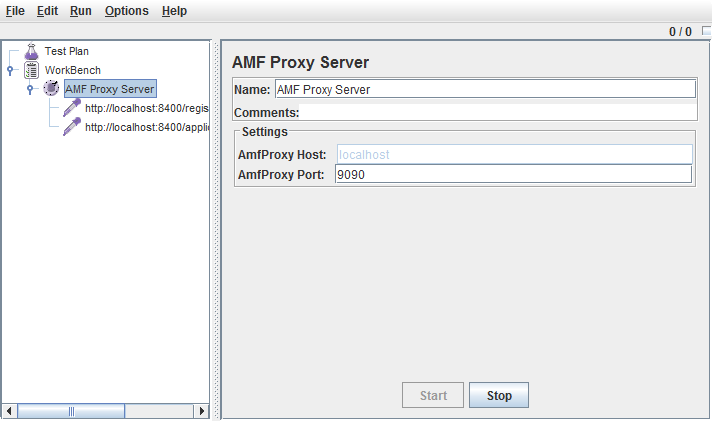
\includegraphics[height=120mm, width=160mm]{fig/development/proxyStart.png}}
\caption{Запуск прокси-сервера}
\label{ris:proxyStart.png}
\end{figure}

\item В AMF RPC Sampler записаны верные параметры AMF запроса, а именно:

\begin{enumerate}
\item Endpoint Url - URL, по которому отправлялся запрос;
\item AMF Call - имя удалённого объекта и процедуы(Например, если мы хоти вызвать у объекта registrationDestionation метод registerUser,
в этом поле следует написать registrationDestination.registerUser);
\item Request Parameters - параметры, переданные методу.
\end{enumerate}

\begin{figure}[ht]
\center{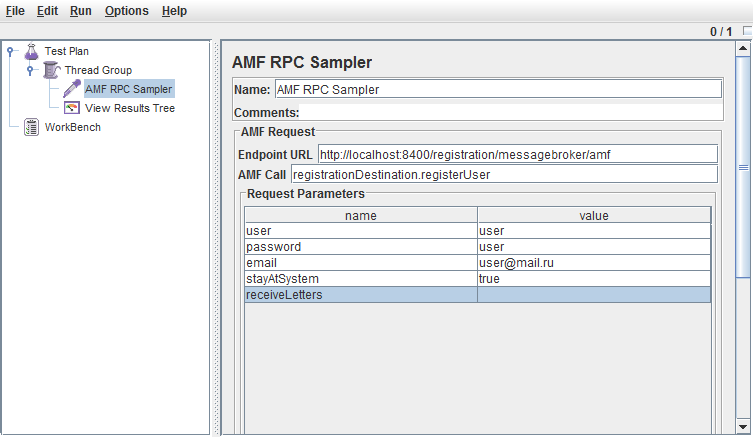
\includegraphics[height=120mm, width=160mm]{fig/development/amfSampler.png}}
\caption{Интерфейс элемента AMF RPC Sampler}
\label{ris:amfSampler.png}
\end{figure}

\end{enumerate}

\subsection{Проверка отправки корректного AMF запроса через AMF RPC Sampler}

Предусловия:

\begin{enumerate}
\item Добавить в Test Plan группу потоков - Thread Group (Test Plan > Threads (Users) > Thread Group).

\begin{figure}[ht]
\center{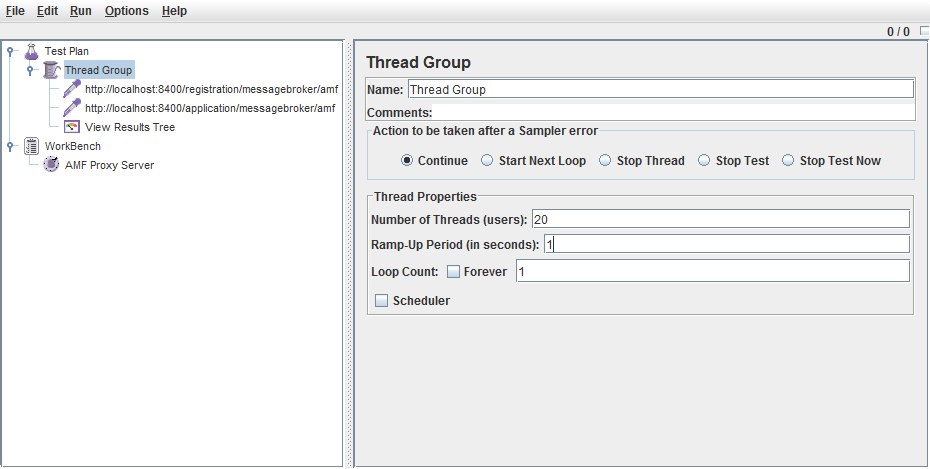
\includegraphics[height=120mm, width=160mm]{fig/development/testplan.png}}
\caption{Создание группы потоков}
\label{ris:testplan.png}
\end{figure}

\item Задать для Thread Group следующие параметры:

\begin{enumerate}
\item Действие, которое будут производиться в случае, если в тест выполняется с ошибкой
(Action to be taken after a Sampler error) --- Continue ;
\item число потоков, в которое будут запускаться шаги тест-плана (Number of Threads) установить равным единице;
\item Интервал, в течение которого будет запущено указанное в предыдущем параметре
число потоков (Ramp-Up Period) установить равным единице;
\item Число повторений набора тестов (Loop Count) установить равным единице;
\end{enumerate}

\item добавить визуалайзер результатов, чтобы иметь возможность отслеживать ход выполнения теста (Thread Group >
Add > Listener > View Results Tree)
\end{enumerate}

Шаги теста:

\begin{enumerate}
\item В Thread Group в качестве дочернего элемента добавить AMF RPC Sampler;
\item Ввести в AMF RPC Sampler все необходимые корректные параметры и запустить содержимое элемента Test Plan (Run > Start);
\item C помощью браузера ввести те же самые данные во Flex приложение и вызвать метод удалённого объекта.
\end{enumerate}

Ожидаемый результат:

\begin{enumerate}
\item После завершения прогона тестов во View Results Tree в дереве элементов тест плана элемент AMF RPC Sampler
посдвечен зелёным цветом (выполнен успешно);
\item на вкладках View Results Tree присутствуют данные запроса и полученного от сервера ответа;
\item Ответ сервера должен быть тем же, что был получен во время вызова процедуры через браузер.
\end{enumerate}

\begin{figure}[ht]
\center{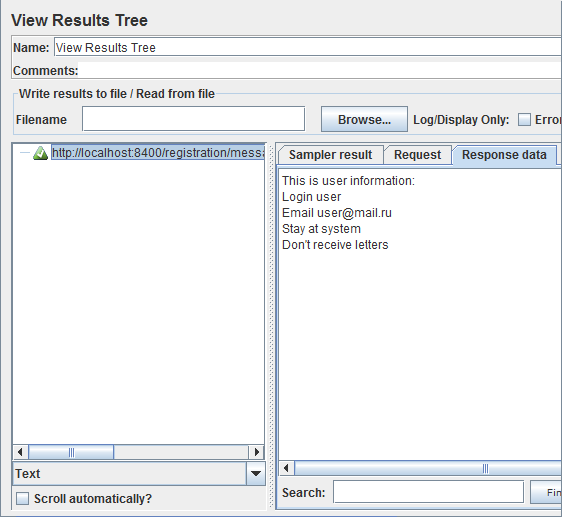
\includegraphics[height=120mm, width=160mm]{fig/development/positiveTest.png}}
\caption{Результаты корректного теста}
\label{ris:positiveTest.png}
\end{figure}

\subsection{Проверка отправки некорректного AMF запроса через AMF RPC Sampler}

Предусловия:

\begin{enumerate}
\item Добавить в Test Plan группу потоков - Thread Group (Test Plan > Threads (Users) > Thread Group).
\item Задать для Thread Group следующие параметры:

\begin{enumerate}
\item Действие, которое будут производиться в случае, если в тест выполняется с ошибкой
(Action to be taken after a Sampler error) --- Continue ;
\item число потоков, в которое будут запускаться шаги тест-плана (Number of Threads) установить равным единице;
\item Интервал, в течение которого будет запущено указанное в предыдущем параметре
число потоков (Ramp-Up Period) установить равным единице;
\item Число повторений набора тестов (Loop Count) установить равным единице;
\end{enumerate}

\item добавить визуалайзер результатов, чтобы иметь возможность отслеживать ход выполнения теста (Thread Group >
Add > Listener > View Results Tree)
\end{enumerate}

Шаги теста:

\begin{enumerate}
\item В Thread Group в качестве дочернего элемента добавить AMF RPC Sampler;
\item Ввести в AMF RPC Sampler неверное имя метода удалённого объекта и запустить содержимое элемента Test Plan (Run > Start);
\end{enumerate}

Ожидаемый результат:

\begin{enumerate}
\item После завершения прогона тестов во View Results Tree в дереве элементов тест плана элемент AMF RPC Sampler
подсвечен красным цветом (тест не пройден);
\item на вкладках View Results Tree присутствуют данные запроса и полученного от сервера ответа;
\item Ответ сервера должен содержать сообщение о соответсвующей ошибке.

\begin{figure}[ht]
\center{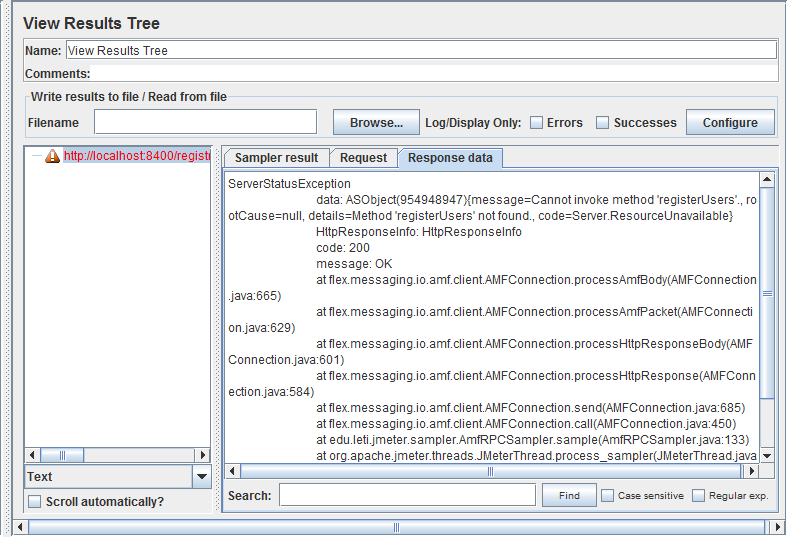
\includegraphics[height=120mm, width=160mm]{fig/development/negativeTest.png}}
\caption{Результаты некорректного теста}
\label{ris:negativeTest.png}
\end{figure}

\end{enumerate}

\subsection{Проверка запуска содержимого Test Plan в несколько потоков}

Предусловия:

\begin{enumerate}
\item Добавить в Test Plan группу потоков - Thread Group (Test Plan > Threads (Users) > Thread Group).
\item Задать для Thread Group следующие параметры:

\begin{enumerate}
\item Действие, которое будут производиться в случае, если в тест выполняется с ошибкой
(Action to be taken after a Sampler error) --- Continue ;
\item число потоков, в которое будут запускаться шаги тест-плана (Number of Threads) установить равным десяти;
\item Интервал, в течение которого будет запущено указанное в предыдущем параметре
число потоков (Ramp-Up Period) установить равным единице;
\item Число повторений набора тестов (Loop Count) установить равным единице;
\end{enumerate}

\item добавить визуалайзер результатов, чтобы иметь возможность отслеживать ход выполнения теста (Thread Group >
Add > Listener > View Results Tree)
\end{enumerate}

Шаги теста:

\begin{enumerate}
\item В Thread Group в качестве дочерних элементов добавить около пяти элементов AMF RPC Sampler;
\item Ввести в элементы AMF RPC Sampler все необходимые корректные параметры и запустить тест план;
\end{enumerate}

Ожидаемый результат:

 После завершения прогона тестов во View Results Tree в дереве элементов все тесты должны быть пройдены ---
 корректный ответ от сервера должен быть получен для каждого элемента.



\end{document}